% !Mode:: "TeX:UTF-8"
\documentclass{../../common/tufte-latex/tufte-handout}

\title{Git en Pratique, partie I: Introduction \& Installation}
\author{S\'ebastien Dawans}

%\date{21 January 2014} % without \date command, current date is supplied

%\geometry{showframe} % display margins for debugging page layout
\usepackage[utf8]{inputenc}
\usepackage{graphicx} % allow embedded images
  \setkeys{Gin}{width=\linewidth,totalheight=\textheight,keepaspectratio}
  \graphicspath{{graphics/}} % set of paths to search for images
\usepackage{amsmath}  % extended mathematics
\usepackage{booktabs} % book-quality tables
\usepackage{units}    % non-stacked fractions and better unit spacing
\usepackage{multicol} % multiple column layout facilities
\usepackage{lipsum}   % filler text
\usepackage{fancyvrb} % extended verbatim environments
  \fvset{fontsize=\normalsize}% default font size for fancy-verbatim environments
\usepackage{listings}
\lstset{showstringspaces=false}
\usepackage[usenames]{xcolor}
\usepackage{hyperref}

\lstdefinestyle{BashInputStyle}{
  language=bash,
  basicstyle=\footnotesize\ttfamily,
  %numbers=left,
  %numberstyle=\tiny,
  %numbersep=3pt,
  frame=tb,
  columns=fullflexible,
  backgroundcolor=\color{yellow!20},
  linewidth=0.95\linewidth,
  xleftmargin=0.05\linewidth,
  moredelim=**[is][\color{red}]{§}{§},
  moredelim=**[is][\color{OliveGreen}]{`}{`}
}

% Standardize command font styles and environments
\newcommand{\doccmd}[1]{\texttt{\textbackslash#1}}% command name -- adds backslash automatically
\newcommand{\docopt}[1]{\ensuremath{\langle}\textrm{\textit{#1}}\ensuremath{\rangle}}% optional command argument
\newcommand{\docarg}[1]{\textrm{\textit{#1}}}% (required) command argument
\newcommand{\docenv}[1]{\textsf{#1}}% environment name
\newcommand{\docpkg}[1]{\texttt{#1}}% package name
\newcommand{\doccls}[1]{\texttt{#1}}% document class name
\newcommand{\docclsopt}[1]{\texttt{#1}}% document class option name
\newenvironment{docspec}{\begin{quote}\noindent}{\end{quote}}% command specification environment



\begin{document}

\maketitle% this prints the handout title, author, and date

\begin{abstract}
\noindent
Ce document introduit Git, un outil de gestion de code source (en anglais: Source Code Management, SCM), et fourni des instructions d'installation à préparer avant la première séance dans le cadre de formations organisées par UseGit.com \marginnote{\color{blue}\underline{\url{http://www.usegit.com}}}.

Le but des cours est d'offrir une première expérience pratique avec Git côté client en utilisant la ligne de commande. \marginnote{Les slides et le matériel de formation sur disponibles sur {\color{blue}\underline{\url{https://github.com/sdawans/git-slides}}}}
Le public cible pour la session est l'un ou plusieurs développeurs ayant déjà reçu une introduction à Git et aux concepts de base tels que ceux fournis dans les slides disponibles publiquement sur le repostory git-slides. 
\end{abstract}

%\printclassoptions

\section{Introduction}\label{sec:intro}

Git est un outil de gestion de code source (SCM) avec trois principes de base.
Git est \textbf{Distribué}, \textbf{Rapide} et \textbf{Fiable}.
Il est très différent de non seulement les outils centralisés comme SVN, mais aussi des autres SCMs distribués comme Mercurial.
Pour mieux suivre cette séance introductive, il est préférable d'oublier les autres SCMs, y compris le vocabulaire qu'ils emploient, car certains fausses similitudes peuvent être déroutantes au début.

\section{Installation: Git en ligne de commande}

En préparation à cette formation, chaque participant devra installer un client Git en ligne de commande et configurer l'accès vers des repository Git hébergés sur un gestionnaire Git local tel que Gitlab ou Gitolite.

Bien qu'il existe plusieurs clients graphiques pour Git tels que SourceTree, SmartGit, Tower, etc, je préfère donner des cours en ligne de commande, et ce pour pluseurs raisons:

\begin{enumerate} 
 \item{\textbf{Les GUIs cachent les commandes Git de base}. Devenir à l'aise avec Git requiert une certaine maîtrise du fonctionnement de l'outil. Afin de se familiariser avec le vocabulaire de base, il est préférable d'utiliser des commandes qui manipulent ce vocabulaire sans couche d'abtraction.}
 \item{\textbf{Les GUIs automatisent certaines opérations}. 
 \marginnote{Cela est particulièrement vrai lorsqu'on aborde les submodules - il est pratiquement impossible d'apprendre le fonctionnement des submodules sans ligne de commande} 
 Les GUIs combient parfois plusieurs opérations Git en une. Cela peut convenir pour certains usages mais au prix de flexibilité et moyens de debug.}
 \item{\textbf{Les GUIs ne vous dépanneront pas}. 
 \marginnote{Lorsqu'on me demande de l'aide avec Git, je commence systématiquement pour ouvir un ligne de commande}
 De temps à autre, même l'utilisateur Git le plus assidu rencontrera des situations inattendues. D'après mon expérience, il est bien plus simple d'analyser et résoudre une telle situation depuis une console que derrière un GUI.}
 \item{\textbf{C'est plus facile en group}. Plus simplement, le fait de suivre une formation données en ligne de commande permet à chacun d'utiliser exactement la même interface. Cela garanti une expérience uniforme dans le groupe.}
\end{enumerate}

Cela dit, une client graphique pourra tout de même améliorer votre productivité plus tard, lorsque vous serez à l'aise avec les commandes de base.

\subsection{Installer un Git client sur MacOS X et Linux}

Les utilisateurs Linux et MacOS X trouveront un client git natif dans leur gestionnaire de dépôt.

Sur certaines distributions Linux, le client git n'est pas toujours très à jour par rapport aux binaires Windows. \marginnote{\url{https://git-scm.com/book/en/v2/Getting-Started-Installing-Git}} donc il peût-être utile d'installer la version la plus récente depuis les sources. Cela n'est cepedant pas nécessaire pour suivre la formation.

\subsection{Installer un Git client sur Windows}\label{sec:preparation}

Les utilisateurs Windows doivent installaer la dernière version de TortoiseGit \marginnote{\url{http://code.google.com/p/tortoisegit/}} (uniquement pour le binaire TortoisePlink.exe) and msysgit \marginnote{\url{http://code.google.com/p/msysgit/}}, dans cet ordre.
Par ailleurs, les utilisateur windows devront installer puttygen.exe et pageant.exe, disponible sur le site de Putty \marginnote{\url{http://www.putty.org/}}. Ceux-ci doivent être stockés à un emplacement connu. En générale, je les place dans 

\begin{lstlisting}[style=BashInputStyle]
  C:\bin\ssh\
\end{lstlisting}

\begin{itemize}

\item{Une pair de clés SSH doit être générée avec puttygen}
\item{La clé publique affichée dans la fenêtre puttygen doit être copié/collée dans la configuration de compte utilisateur sur votre gestionnaire Git (Github, Gitlab, Gitolite, Redmine...) tandis que la clé privée devra être enregisrée sur votre PC et ajoutée à Pageant} \marginnote{Losque vous copiez votre clé publique dans GitLab / Redmine, etc, assurez-vous de bien copier depuis le GUI puttygen et non pas depuis le fichier de clé publique. Cela évite une erreur fréquemment rencontrée lorsqu'on fourni un clé qui n'est pas en format OpenSSH.}
\item{Optionnellement, vous pouvez créer un script batch qui lance pageant.exe au démarrage de votre machine et qui y ajoute automatiquement la clé privée.}
\item{Créez une nouvelle variable d'environnement Windows nommée GIT\_SSH et pontant sur TortoisePlink.exe, installé avec TortoiseGit:}
\begin{lstlisting}[style=BashInputStyle]
  GIT_SSH = C:\Program Files\TortoiseGit\bin\TortoisePlink.exe
\end{lstlisting}
\item{Après la création de cette variable d'environnement, vous devez fermer et rouvrir toute éventuellement console Git. Depuis Git Bash, vérifiez la bonne configuration de GIT\_SSH en tappant:}

\begin{lstlisting}[style=BashInputStyle]
  $ echo $GIT_SSH
  C:\Program Files\TortoiseGit\bin\TortoisePlink.exe
\end{lstlisting}

\end{itemize}

\subsection{Configurer Git}

Git attache beaucoup d'importance aux personnes: chaque changement doit être attribué à un auteur. 
\marginnote{En fait, Git g\`{e}re m\^{e}me deux types d'utilisateur en distinguant les \textbf{authors} des \textbf{committers}}.

L'auteur est la personne qui est à l'origine d'un certain patch (nouveau code, modification de code), tandis que le committer est la personne qui a appliqué ce changement à un certain moment dans l'historique du projet.

Un utilisateur doit donc s'indentifier avant d'utiliser son client Git.
Git utilise des variables globales \texttt{user.name} et \texttt{user.email} appliqué à tous les projets et pouvant être redéfini au niveau d'un repository particulier.
Pour cette session, nous allons utiliser une configuration globale au client Git:

\begin{lstlisting}[style=BashInputStyle]
  $ git config --global user.name "Prenom Nom"
  $ git config --global user.email "prenom.nom@example.com"
\end{lstlisting}

Une autre configuration utile (déjà activée par défaut sur msysgit) est l'activation des couleurs dans l'output de Git:

\noindent To do so:

\begin{lstlisting}[style=BashInputStyle]
  $ git config --global color.ui true
\end{lstlisting}

Les utilisateurs Windows qui ne sont pas comfortables avec Vim, l'éditeur de text par défaut dans msysgit, peuvent définir une option \texttt{core.editor}.
Par exemple, pour utiliser Notepad++ comme éditeur préféré:

\marginnote{D'après \url{http://starikovs.com/2012/11/06/git-core-editor-windows/}, vous pouvez écrire simplement 'notepad++' à condition qu'il soit correctement défini dans votre PATH}
\begin{lstlisting}[style=BashInputStyle]
  $ git config --global core.editor
    "'C:/path/to/notepad++.exe' -multiInst -notabbar -nosession -noPlugin"
\end{lstlisting}

A ce stade, il est utile de remarque que les \texttt{git config} ci-dessus utilisent l'option \texttt{--global}  pour stocker la configuration dans un fichier global à l'utilisateur de la machine, stocké dans 

\begin{lstlisting}[style=BashInputStyle]
  ~/.gitconfig
  --> C:\Users\MyLogin\.gitconfig  # Windows
  --> /home/user/.gitconfig        # Linux
\end{lstlisting}

Sans l'option \texttt{--global}, la commande \texttt{git config} applique des configurations localement au repository courant, et écrase la configuration globale du même nom en cas de doublon. Le fichier de configuration locale à un repository se trouve dans:

\begin{lstlisting}[style=BashInputStyle]
  root_folder/.git/config
\end{lstlisting}

\noindent Ces deux fichiers peuvent être ouverts et édités directement avec: \marginnote{Une recherche Google pour \textbf{git dotfile} vous fera décourir un tas d'alias utilisés par d'autres développeurs qui sont utiles à ajouter au fichier de configuration global. Cependant, comme pour les GUIs, nous n'allons pas utiliser d'alias lors de l'apprentissage.}

\begin{lstlisting}[style=BashInputStyle]
  git config [--global] --edit
\end{lstlisting}

\noindent Pour une liste complète de paramètres globaux et redéfinis localement, utilisez

\begin{lstlisting}[style=BashInputStyle]
  $ git config --list
\end{lstlisting}

Enfin, une configuration utile avant de commencer est la \textbf{customisation de prompt.}
Les utilisateurs Windows se servant déjà de msysgit disposent d'une forme basique de prompt customisé. \marginnote{Git Prompt: \url{http://volnitsky.com/project/git-prompt/}}
Pour les système à base d'Unix, je recommende le projet git-prompt.

%TODO: make my notes on git-prompt public and add a link to it

\subsection{Solutions d'hébergement Git recommandées}

Comme la plupart de ces formations sont données en entreprise, il est courant d'aborder les aspects d'hébergement de repository Git.

\textbf{Gitlab}

\marginnote{Mon avis sur Gitlab [FR] \url{https://www.cetic.be/Solution-Open-Source-et-complete-d}}
\begin{marginfigure}%
  \centering
  
\includegraphics[width=0.6\linewidth]{gitlab-logo.png}
  \label{fig:gitlablogo}
\end{marginfigure}

\noindent Gitlab est un gestionnaire Git gratuit open-source et très largement utilisé, offrant un expérience similaire à Github mais ayant l'avantage d'être  hébergé dans l'entreprise et donc entièrement privé.

Gitlab offre une interface web pour la gestion et la visualisation de repository Git hébergés sur le serveur.
Chaque repo hébergé sur Gitlab dispose d'une URL unique, en général \\ \noindent \texttt{http://gitlab.server.com/namespace/project}

Le \textbf{namespace} peut être de deux types: un namespace propre à chaque utilisateur, ou des namespaces de groupes.

Bien que la procédure d'installation officielle de Gitlab renseignée dans le README et très simple à utiliseur, certains utilisateurs opteront plutôt pour des images Gitlab toutes faites, telles que celles fournies par Bitnami. 

\textbf{Redmine + Gitolite}

\begin{marginfigure}%
  \centering
  
\includegraphics[width=0.6\linewidth]{redmine-logo.png}
  \label{fig:gitlablogo}
\end{marginfigure}

\noindent Redmine est un gestionnaire de projet très répandu et qui supporte l'intégration de Gitolite à travers le plugin Redmine Git Hosting \marginnote{Redmine Git Hosting \url{https://www.redmine.org/plugins/redmine_git_hosting}}. Cette installation est plus complèxe que celle de Gitlab et ne doit être suivie que par un sys-admin aguerri.

\subsection{Tester la connexion SSH vers le repository Git}

La denière étape de configuration consiste à vérifier l'état de la connexion au serveur de repos Git.

\begin{marginfigure}%
  \centering
  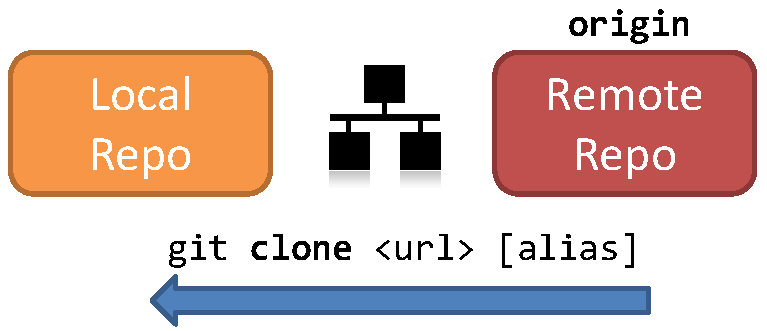
\includegraphics[width=\linewidth]{gitclone-schema.pdf}
  \label{fig:gitclone}
\end{marginfigure}
\marginnote{Un argument supplémentaire peut être fourni poru spécifier le nom du dossier en local}
\marginnote{Le protocole SSH est implicite en utilisant le format d'URL user@server. C'est équivalent à ssh://user@server}
Nous pouvons tenter de \textbf{clone} un repository existant for cela.
En jargon Git, \texttt{clone} consiste à copier un repository complet depuis un serveur distant vers sa machine locale.
Contraitement à des SCMs centralizés comme SVN, \texttt{git clone} par défaut copiera chaque information nécessaire pour reconstituer une quelconque version du projet depuis le début.
C'est pour cela que l'on parle d'un outil distribué: chaque clône est en réalité un repository complet à part entière.

\begin{lstlisting}[style=BashInputStyle]
  $ git clone git@gitlab.server.com:login/lesson1 [folder]
\end{lstlisting}

\noindent Lorsque la connection fonctionne, git clônera le repository et renverra quelques détails sur l'opération:

\begin{lstlisting}[style=BashInputStyle]
  Cloning into 'lesson1'...
  remote: Counting objects: 23, done.
  remote: Compressing objects: 100% (17/17), done.
  remote: Total 23 (delta 3), reused 0 (delta 0)
  Receiving objects: 100% (23/23), done.
  Resolving deltas: 100% (3/3), done.
\end{lstlisting}

Un nouveau répertoire \texttt{lesson1} apparaître dans le dossier courant.
Le repository Git (dossier \texttt{.git}) et le \texttt{working tree} sont tous les deux contenus dans le répertoire \texttt{lesson1}
\marginnote{\texttt{lesson1}, comme tout repository Git, est entièrement autonome et peut être déplacer sur votre machine sans risque.}

\marginnote{Le dossier \texttt{.git} est le repository lui-même avant tous les objets Git et la configuration. Nous n'allons plus nous attarder sur ce dossier durant le reste de la formation.}
\begin{lstlisting}[style=BashInputStyle]
  $ cd lesson1/
  $ tree -L 2 -a 
  .
  |-- .git
  |   |-- branches
  |   |-- config
  |   |-- description
  |   |-- HEAD
  |   |-- hooks
  |   |-- index
  |   |-- info
  |   |-- logs
  |   |-- objects
  |   |-- packed-refs
  |   `-- refs
  |-- python
  |   `-- calc.py
  `-- README.md
\end{lstlisting}

Le \textbf{working tree} est l'ensemble de fichiers et dossiers contenus dans le répertoire \texttt{lesson1}, sans compter le \texttt{.git}.
\begin{marginfigure}%
  \centering
  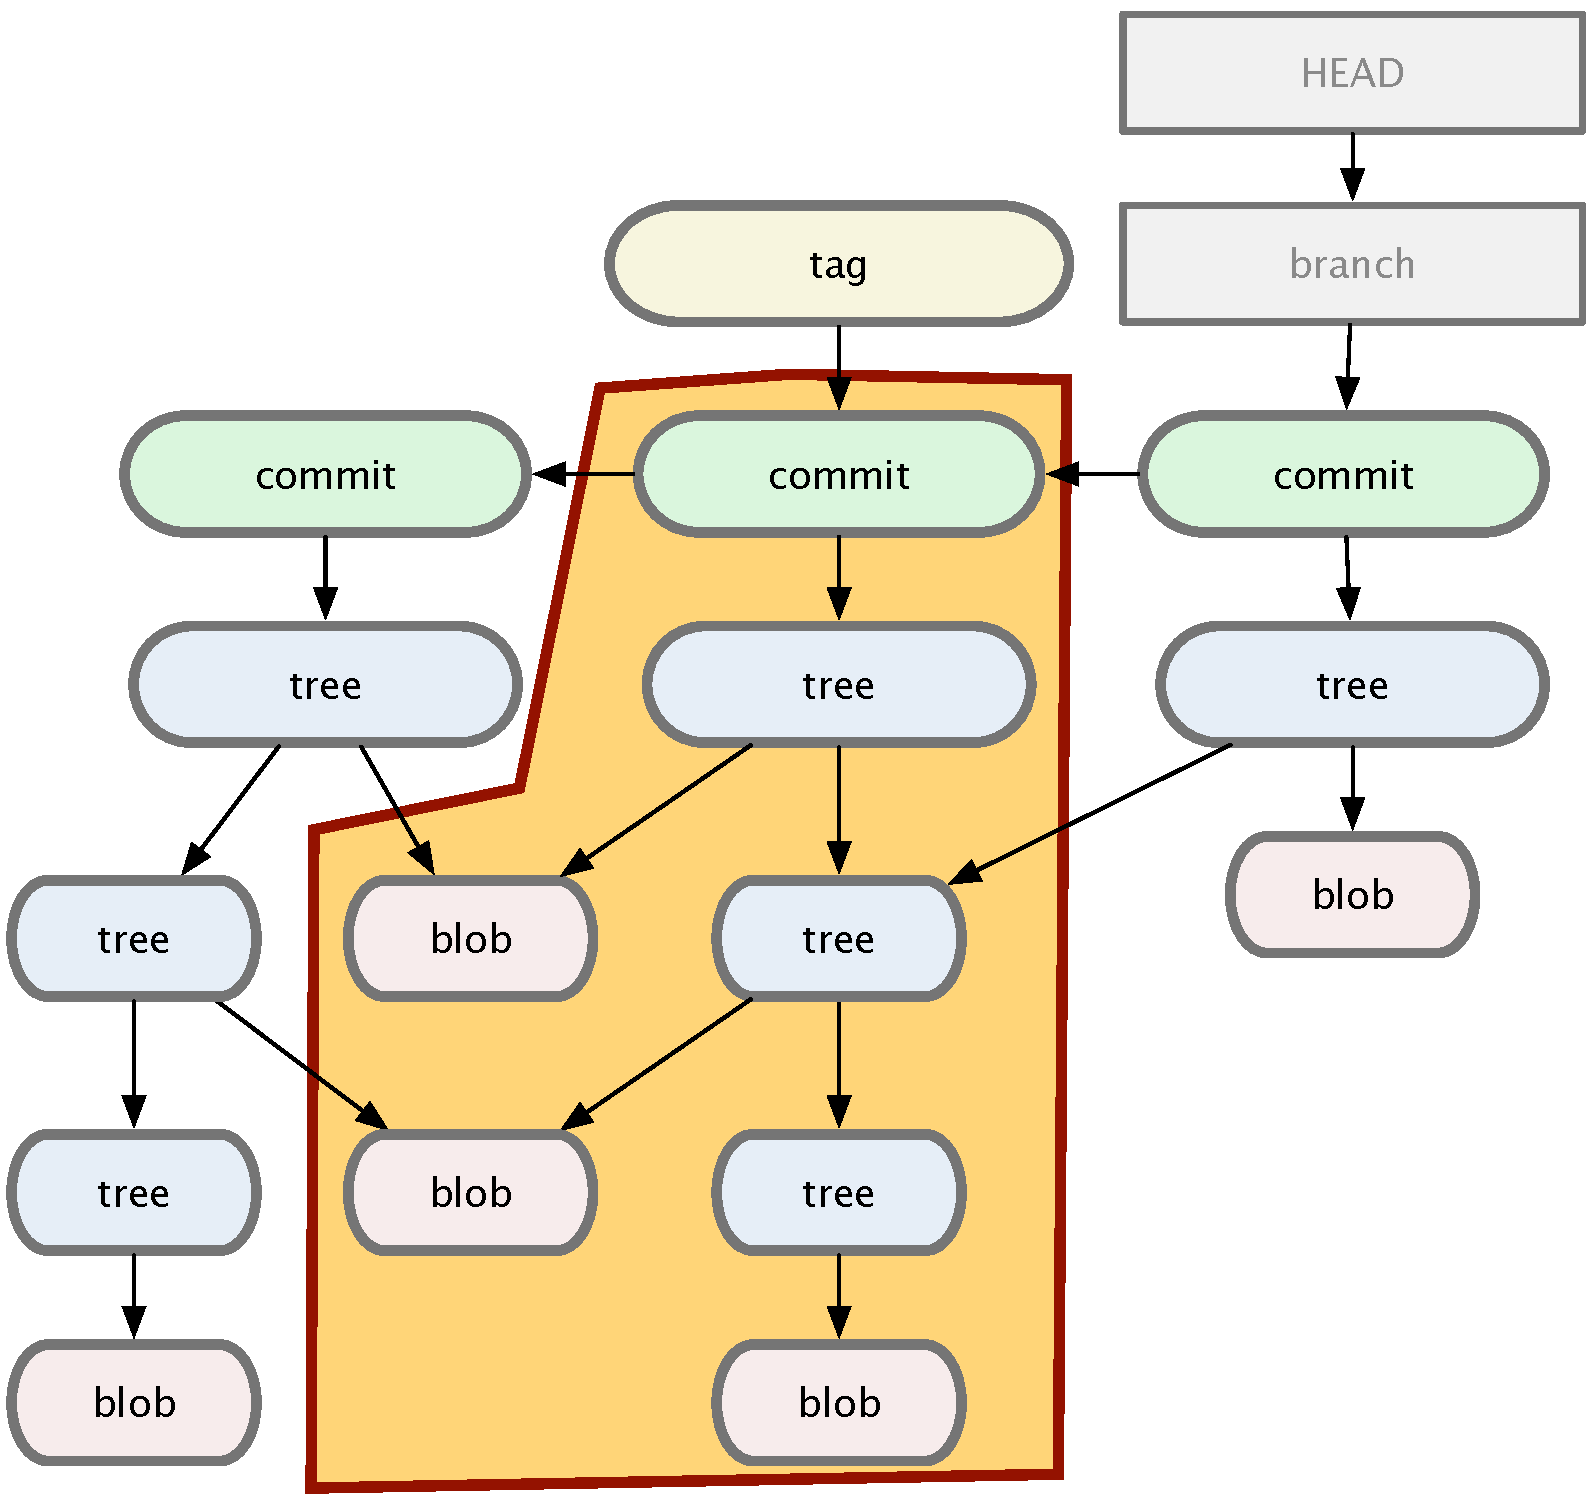
\includegraphics[width=\linewidth]{tree.pdf}
  \label{fig:tree}
  \caption{Représentation d'un working tree arbitraire pour un certain commit. Les fichiers sur disque et leurs dossiers contenants sont représentés par des objets\texttt{blob} et texttt{tree}}
\end{marginfigure}

Dans notre working tree, nous avons un fichier \texttt{README.md} à la racine, et un script python dans un répertoire \texttt{python}
Seule une \textit{version unique} d'un working tree peut être \textit{checked out} ("sur le disque") à la fois.

Comme nous avons déjà vu dans les slides d'introduction, le \texttt{working tree} est un cliché complet du projet à un certain stade de l'historique.
Un version est entièrement désignée par un objet de type \textbf{commit}, contenant un auteur, committer, date et pointant vers le \textbf{tree} racine et l'un ou plusieurs \textbf{commits parents}.
Chaque objet \textbf{tree} est à son tour consistué de \textbf{tree} et de \textbf{blob}, des fichiers.
Ce cours ne couvre pas le fonctionnement interne de Git au delà de ce qui est présenté dans les slides d'introduction.

\section{Lectures complémentaires}

La prochaine leçon \texttt{Partie II: Opérations en solo}, introduit la plupart des commandes Git de base. Elle est conçue de manière à apprendre l'utilisation basique de Git à travers la pratique et en s'affranchissant momentanément de la complexité du travail à plusieurs. Les workflows multi-utilisateurs sont décrits en Partie III.

\bibliography{tufte-latex/sample-handout}
\bibliographystyle{plainnat}



\end{document}
